\chapter{NOGWs excited by tropopause depressions in a 2D plane}
\label{sec:resultsQ3D}
% The sensitivity of 

\begin{tcolorbox}[]
    (R1) How sensitive are NOGWs from propagating tropopause folds to the 2D shape of the depression and the stratospheric environment?
\end{tcolorbox}


% define quasi 3d simulations
Following the results of the model validation / comparison of GWD with linear solutions




\section{Quasi-3D reference Simulation}
\label{sec:resultsq3D-reference}


For the stratosphere the assumption of a two atomic gas  possible to de


\begin{figure*}[tbp]
    \centering
    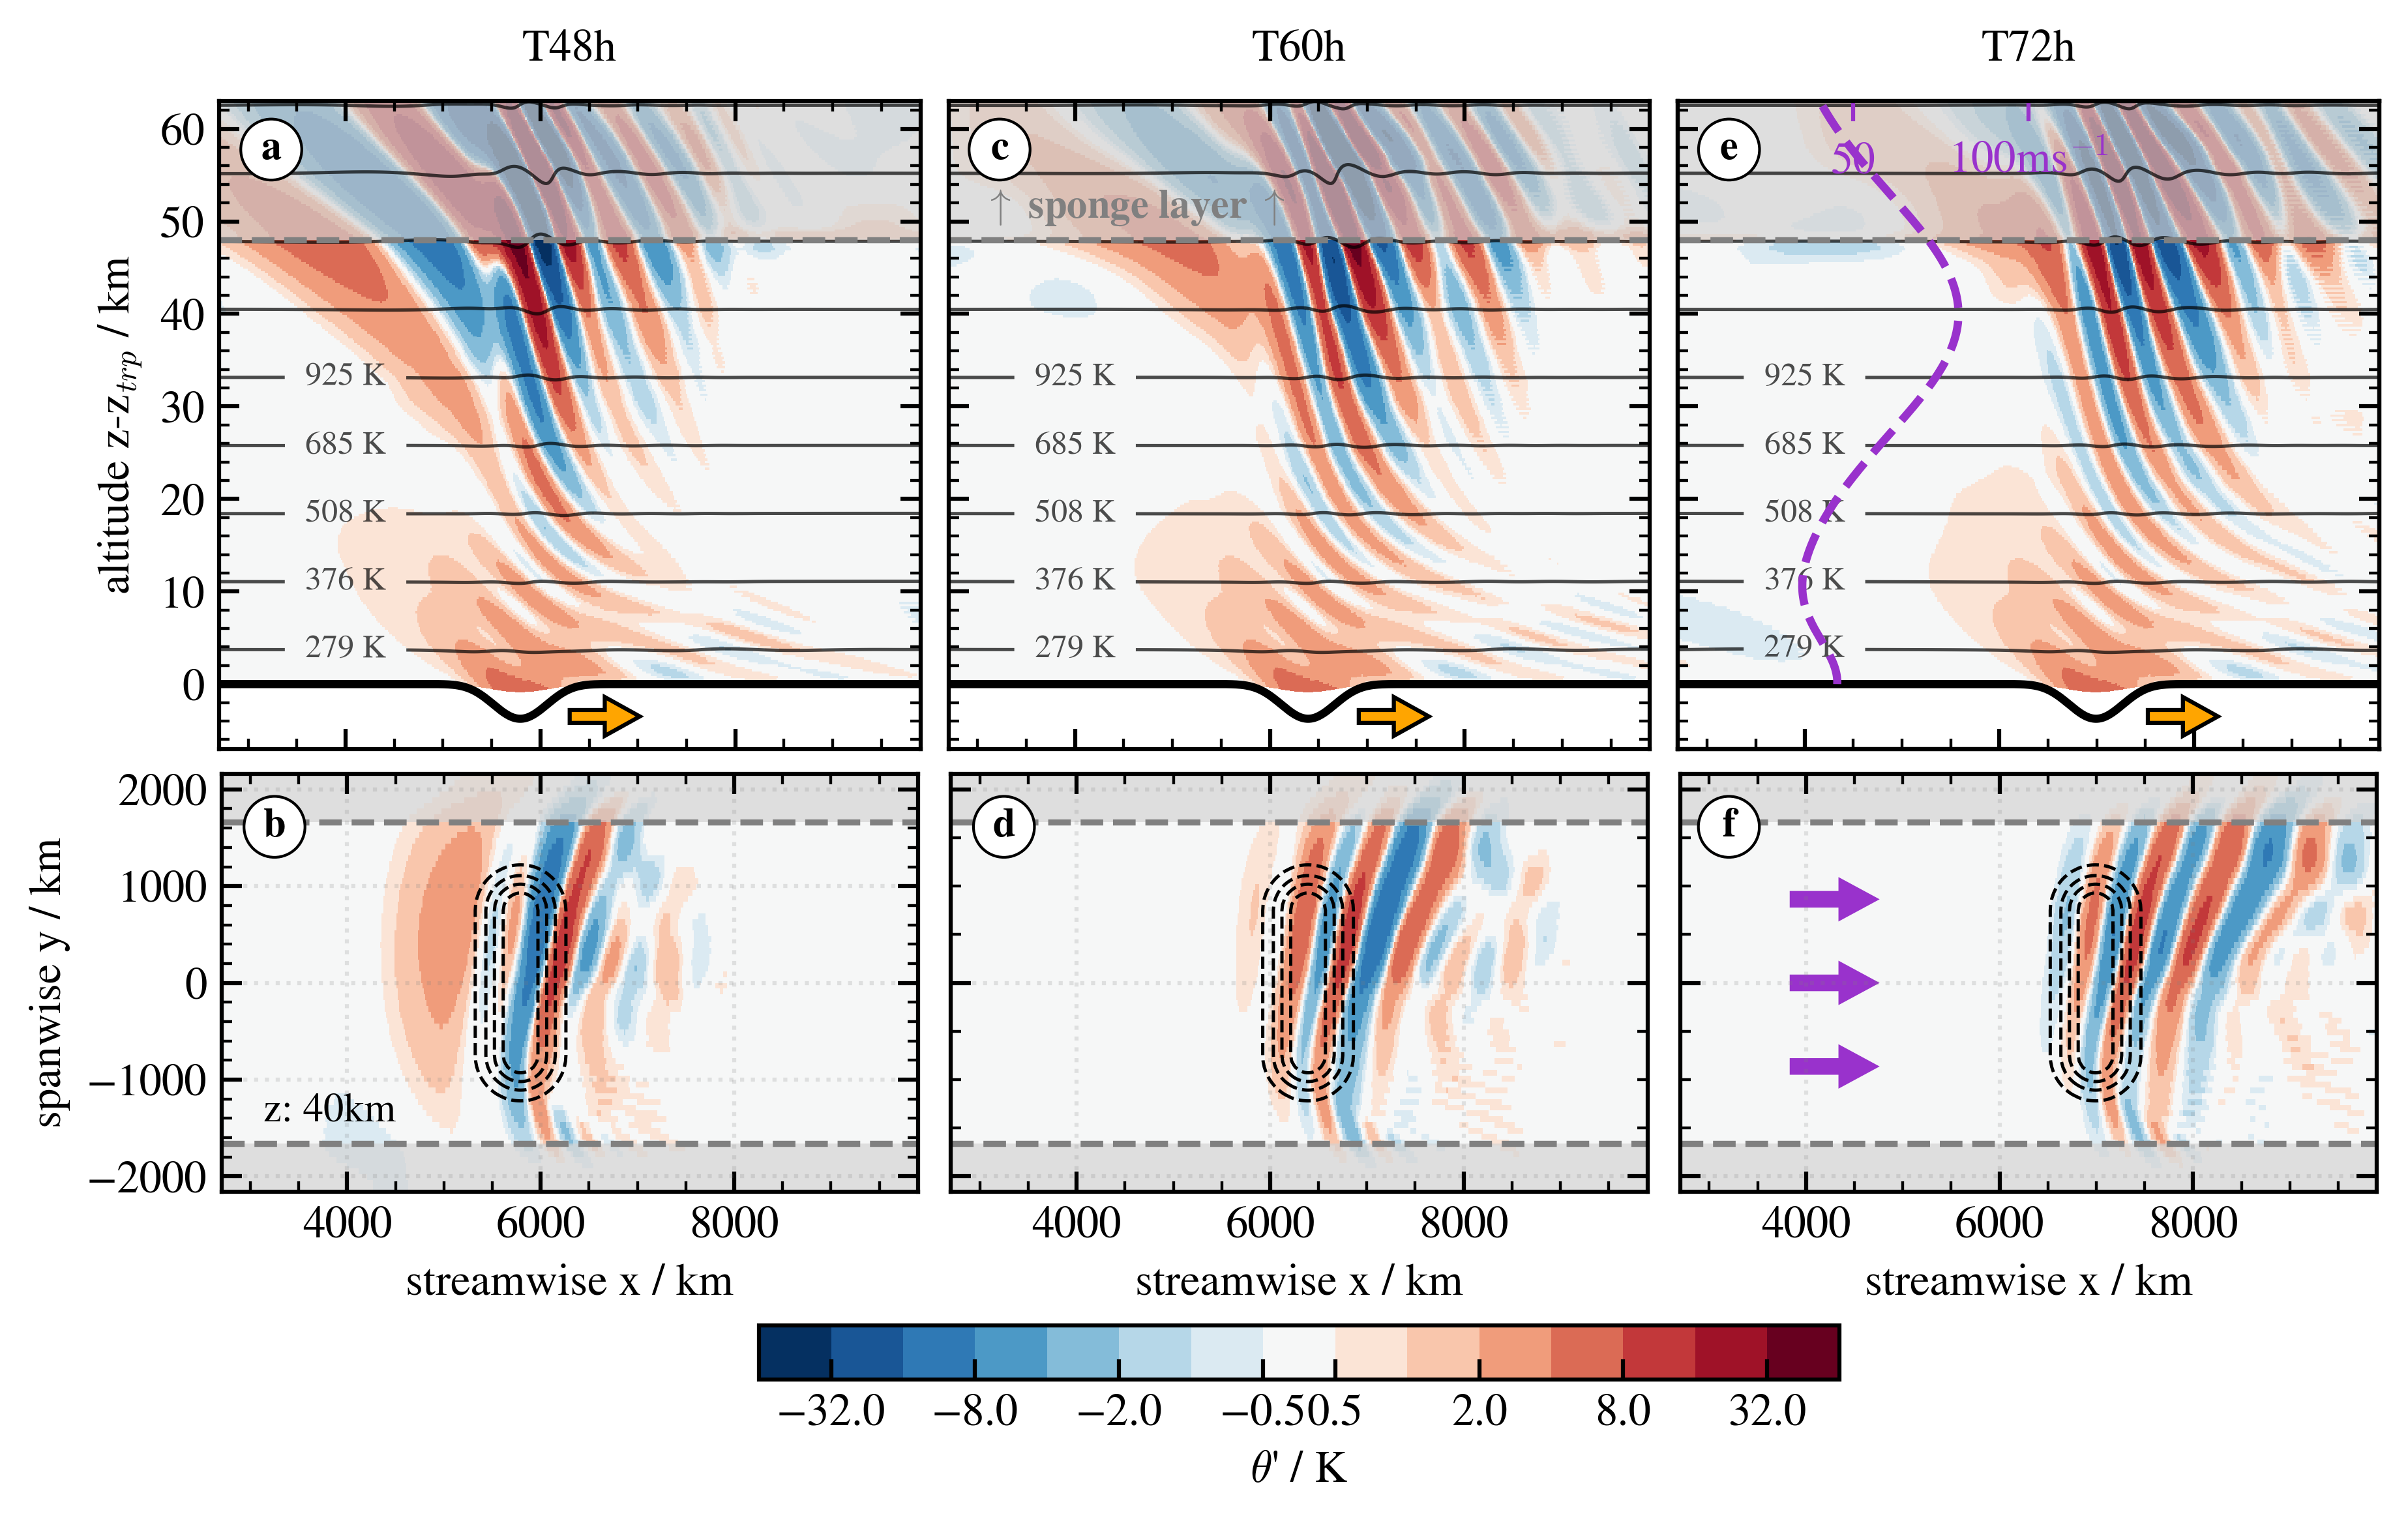
\includegraphics[width=0.99\textwidth]{figures_q3D/Q3D-th-referenceSim.png}
    \caption{Horizontal cross sections at 40km above the tropopause for five simulations with horizontal and meridional shear in a barotropic environment. Shown are $\theta$', $\lambda_x$ and $\lambda_y$ at 72h into the simulation. Dominant zonal and meridional wavelengths for each grid point are determined from wavelet analysis.}
    \label{fig:q3D_referenceSim}
\end{figure*}

\section{Influence of tropopause shape}
\begin{figure*}[tbp]
    \centering
    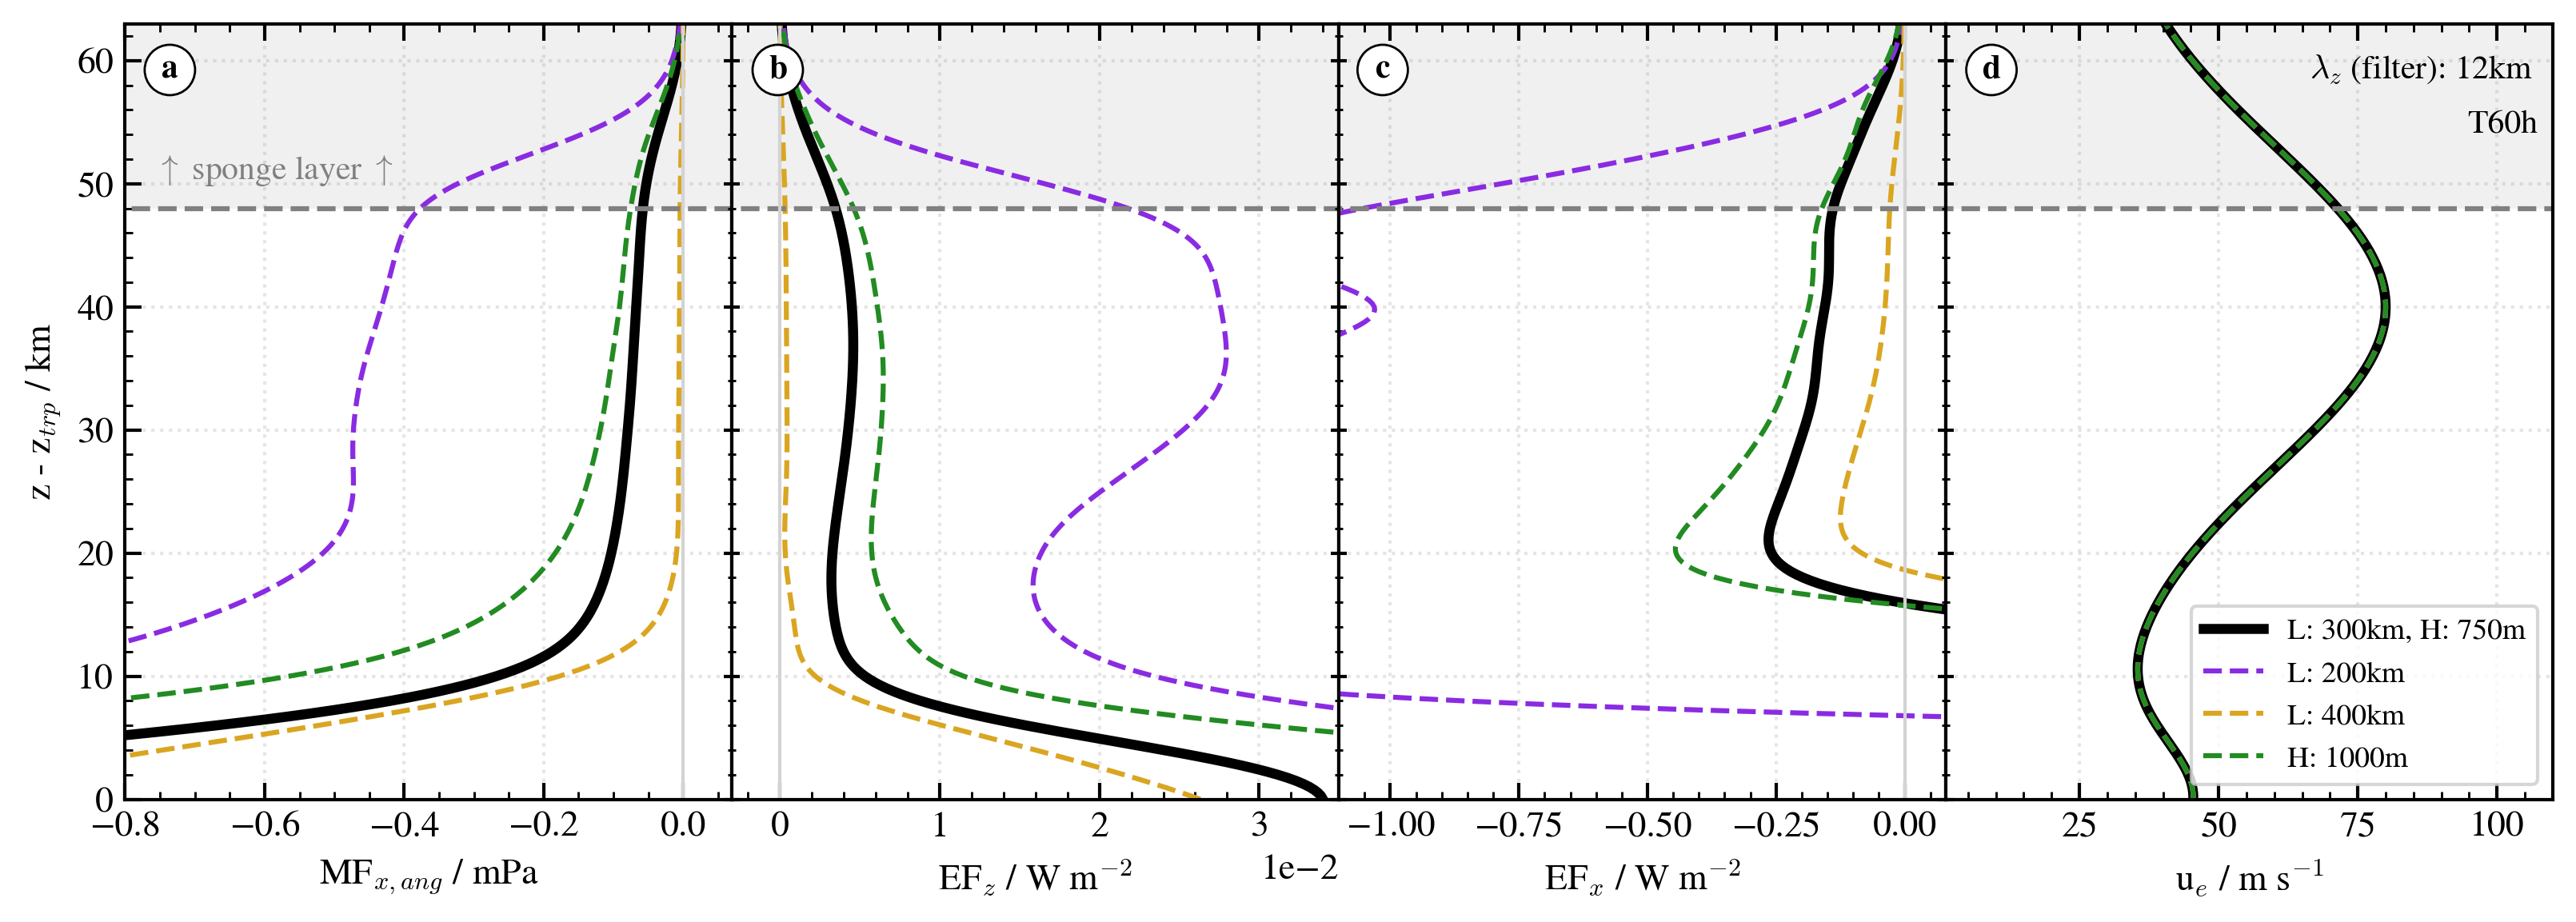
\includegraphics[width=0.99\textwidth]{figures_q3D/TD-zprofiles-translbq3D_shape-T60h-avg.png}
    \caption{Horizontal cross sections at 40km above the tropopause for five simulations with horizontal and meridional shear in a barotropic environment. Shown are $\theta$', $\lambda_x$ and $\lambda_y$ at 72h into the simulation. Dominant zonal and meridional wavelengths for each grid point are determined from wavelet analysis.}
    \label{fig:q3D_shape}
\end{figure*}


\section{Influence of background zonal wind}
\begin{figure*}[tbp]
    \centering
    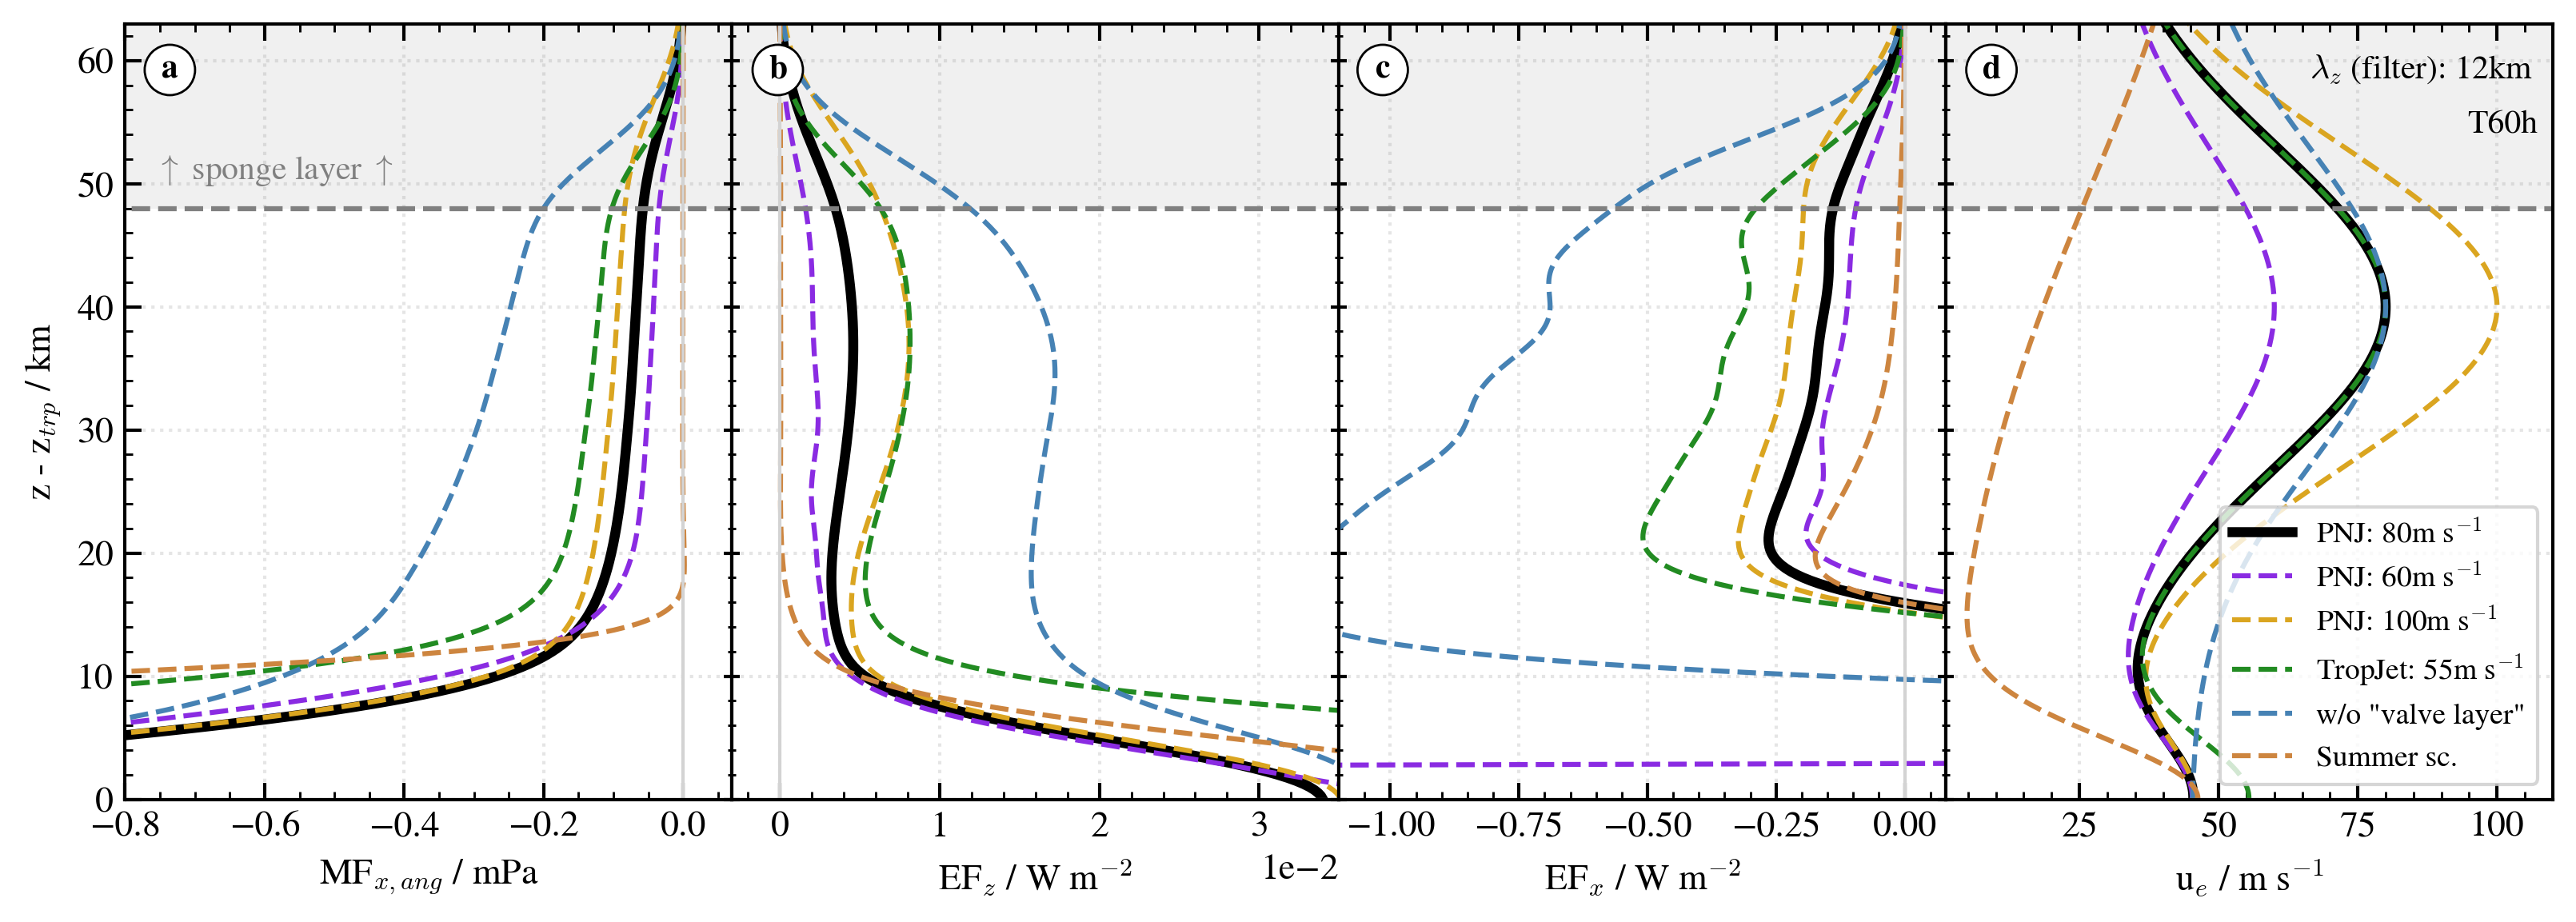
\includegraphics[width=0.99\textwidth]{figures_q3D/TD-zprofiles-translbq3D_wind-T60h-avg.png}
    \caption{Horizontal cross sections at 40km above the tropopause for five simulations with horizontal and meridional shear in a barotropic environment. Shown are $\theta$', $\lambda_x$ and $\lambda_y$ at 72h into the simulation. Dominant zonal and meridional wavelengths for each grid point are determined from wavelet analysis.}
    \label{fig:q3D_wind}
\end{figure*}

% Reflection layers in the presence of the PNJ are relevant for horizontal wavelenghts below 30-\SI{40}{\kilo\meter} (\cite[]{gill_atmosphere-ocean_1982} and Mixa), but less of a concern for the large scale inertia-gravity waves observed in our simulations.

GW starts to dissipate momentum as soon as background environment (wind profile and stability (theta profile)) approaches a critical level. In theory, the momentum is only absorbed at the critical level, but in reality GWs are not even able to reach the critical (vertical wavelength and vertical group velocity vanishes). Thus, the dissipation process should be more understood as an continuous process that starts as soon as the GW approaches a critical level due to changing background conditions. In addition, a three dimensional flow has a continuous spectrum if critical levels due to a turning of the wind with height. 


convective instability vs. shear instability 
check paper andreas norway

Figure --- and ... tell the same story. The absence of a wind minimum above the tropopause jet has the largest effect on the energy fluxes or the vertical flux of horizontal momentum. Though wind speeds at the tropopause level or the altitude of the PNJ are similar to the reference simulation, the flux towers in Figure ... and the zonal averages in figure ... show significantly higher values for the simulation without negative shear above the tropopause jet. How can this phenomenon be explained in the context of significant publications (\cite[]{eliassen_transfer_1960} or \cite[]{bretherton_momentum_1969}) that consider dissipation only in the context of a critical level. 

%Varying wind speeds with altitude could lead to critical levels. An internal gravity wave reaches a critical level when its horizontal phase speed $c_{p,x}$ is equal to the background wind. This results in a vanishing intrinsic frequency or for inertia-gravity waves in an inertial oscillation with $\hat{\omega}=f$. In the case of stationary mountain waves $c_{p,x}$ and a critical levels exists when U(z)=0. For the propagating tropopause fold $c_{p,x}=c_{tf}=\SI{13.88}{\meter\per\second}$ considering the MW like behaviour within the moving reference frame. Thus, 

Layers of reReflection layers have already been ruled out, 

% inertial critical levels, where Uk = ±f (or in general Uk + Vl = ±f). Jones found that in rotating flow it is the wave angular momentum
\textcite[]{teixeira_physics_2014} 


% However, the interest for flows with directional shear and critical layers (where the wave momentum is deposited over a continuous range of heights, as opposed to critical levels) has increased recently, since these flows are much more realistic
cite teixeira 2009

% Additionally, Eliassen-Palm's theorem states that, in the same circumstances, the momentum flux is constant with height except at critical levels (Broad 1995)

% For a directionally sheared flow and a 3D mountain, there is no single critical level, but a distribution of them with height, depending on the wavenumber of the gravity waves (i.e., a critical layer). This study aims to calculate the momentum flux in such situations of directional shear and 3D orography, addressed first by SG99

% According to Eliassen and Palm [1960] for linear, steady, small-amplitude, non-dissipative MW   !!! −𝐸𝐹 = 𝑢𝑀𝐹𝑥 + 𝑣𝑀𝐹𝑦 !!!


%Dissipation results from processes such as radiative damping [Fels, 1984; Zhu, 1994], wave–wave and wavemean flow interactions [Broutman and Grimshaw, 1988; Sutherland, 2000, 2001], and wave breaking and instability processes (see section 6).
fritts 2003

flux of angular momentum stays constant for IGWs.

\textcite[]{kruse_midlatitude_2016} obser

\textcite[]{kruse_gravity_2015} 

% Another important constraint on steady, linear moun- tain waves is the conservation of momentum flux with height with background wind shear (Eliassen and Palm 1960). According to Eq. (9), EFz will vary with height proportionately with u(z). Physically, this variation in EFz is caused by a conversion from mean-state shear energy to wave energy flux according to [from Eq. (9)]
% dEFz 52MFdu. (11) dz dz


% This mountain wave valve layer is distinct from a critical level. A critical level is defined as the level where the ambient wind speed through a wave (i.e., wind speed perpendicular to the phase fronts U?) is equal to the horizontal phase speed cp of the gravity wave. For a north–south-oriented stationary mountain wave (U? 5 U, cp 5 0), a critical level is a level of zero ambient zonal wind. Mountain waves of all amplitudes and scales will be almost completely attenuated at a zonal wind reversal (i.e., critical level) in this scenario (Booker and Bretherton 1967). A valve layer, however, is defined as a layer of reduced wind speed with no wind reversal or critical level (e.g., Fig. 9). Such a layer might allow small-amplitude mountain waves to be trans- mitted unaffected but might also cause larger-amplitude mountain waves to steepen, become nonlinear, and at- tenuate (e.g., between 23 June and 5 July in Figs. 8a,e,g). The valve-layer concept may also be applied to non- stationary gravity waves (i.e., cp 61⁄4 0) by consider- ing profiles of wind speed through the wave relative to the wave phase speed (U? 2 cp). Wave attenua- tion within this frequently present lower-stratospheric valve layer above New Zealand is quantitatively in- vestigated below.

However, MFx
above the valve layer is primarily controlled by the mini-
mum wind speed within the valve layer alone 


Mountain waves were strongly and nonlinearly attenuated in the valve layer above this jet,

This theoretical limit is never achieved in the real atmosphere because a host of instability and dissipation mechanisms become more likely as a wave approaches a critical level. \cite[]{fritts_gravity_2003}



\begin{equation}
    c_{gx} \approx \frac{N^2 \alpha}{m \sqrt{f^2+N^2 \alpha^2}} \approx \SI{-26.9}{\meter\per\second} 
    %\label{}
    % (phase propagation against the background wind results in a negative horizontal scale $k$ and, thus, negative $\alpha$)
\end{equation}
with a negative $m$ for upward propagating waves and the vertical group velocity
\begin{equation}
    c_{gz} \approx -\alpha c_{gx} \approx \SI{0.36}{\meter\per\second}
    % \label{equ_lid:cgz}
\end{equation}


\section{Influence of Coriolis force and stratification}
% make one section



\section{The influence of the fold's propagation speed}
% difference due to rising mountain?? 
\begin{figure*}[tbp]
    \centering
    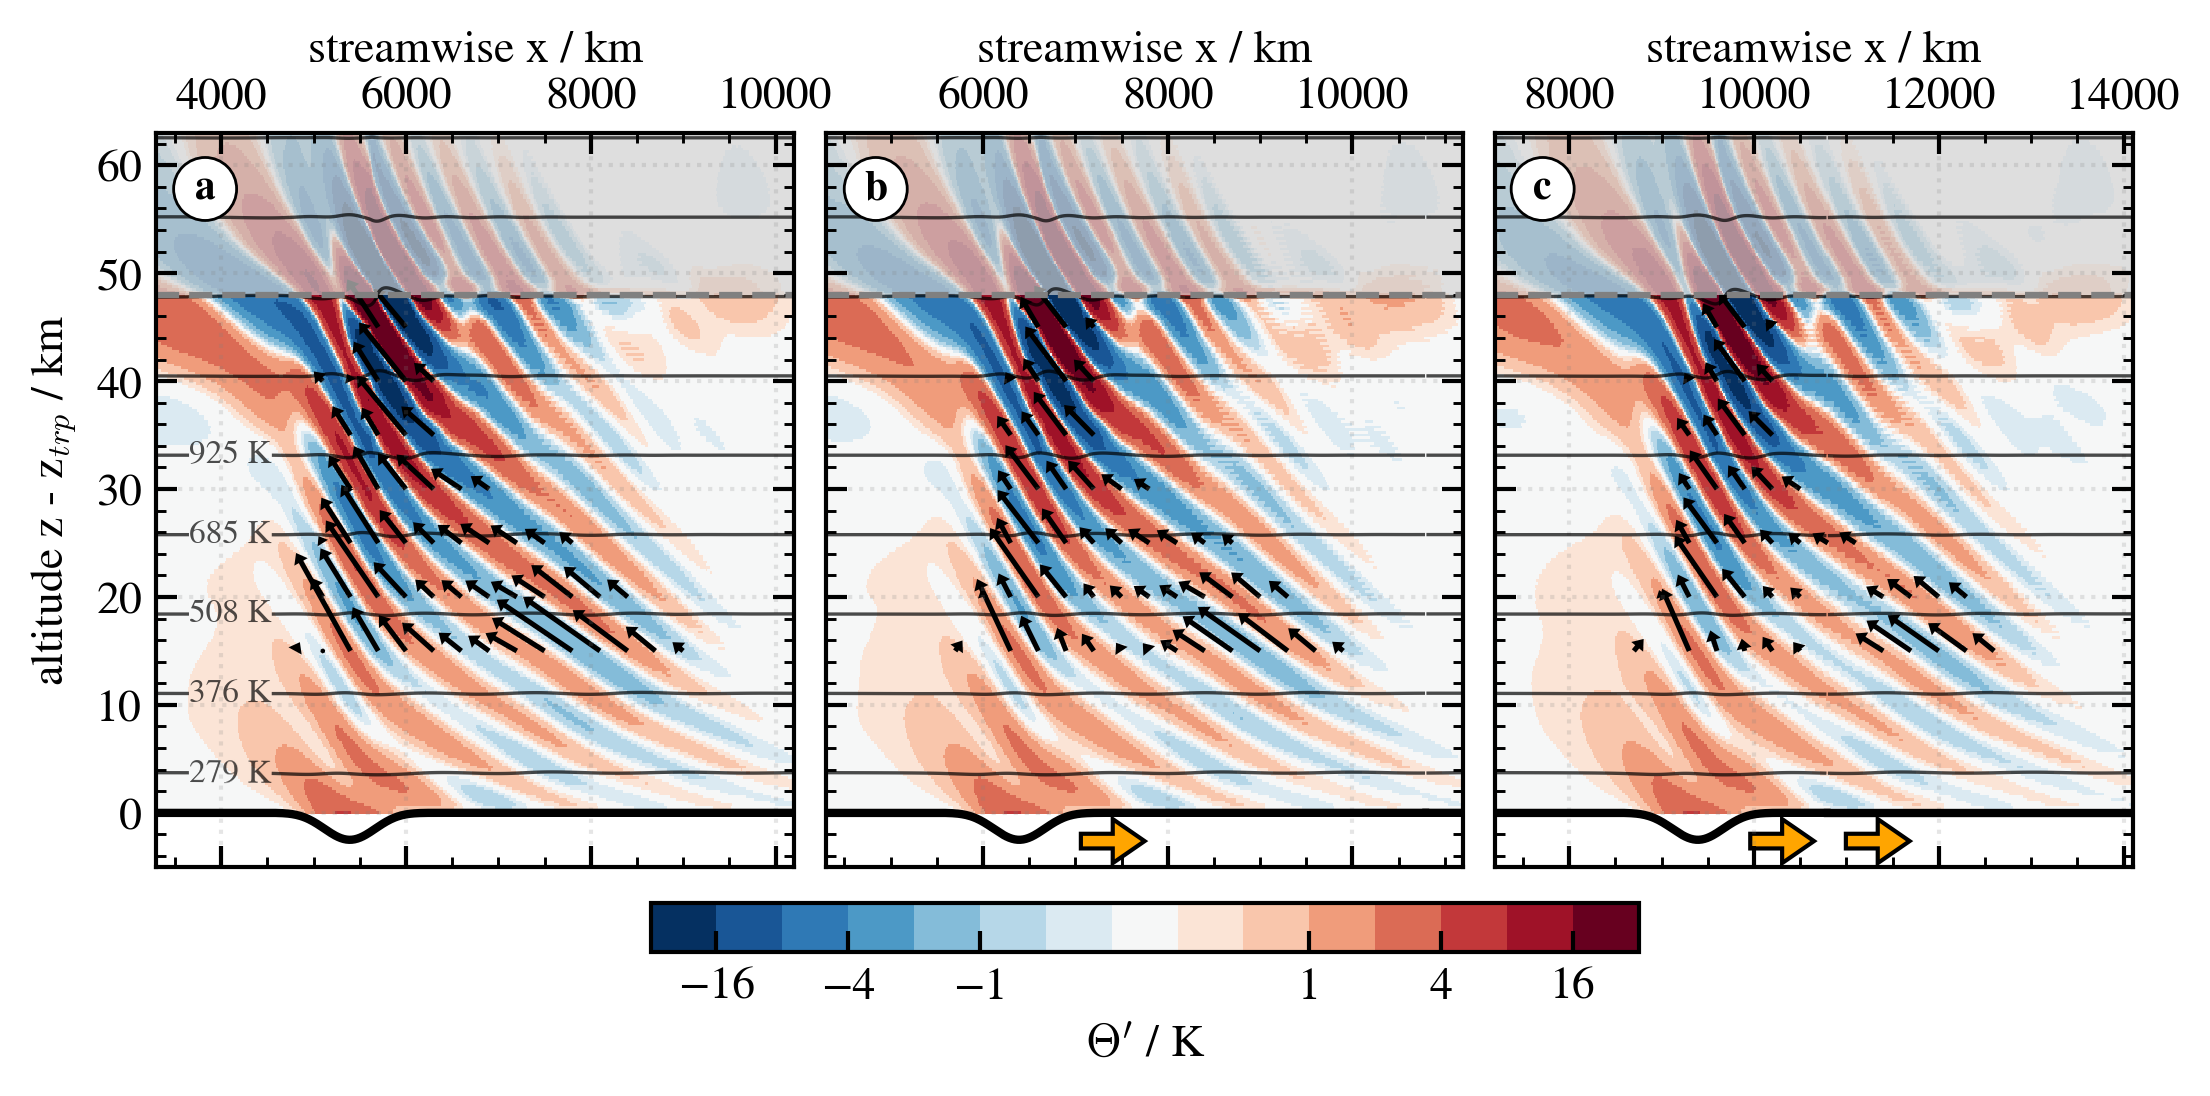
\includegraphics[width=0.99\textwidth]{figures_q3D/Q3D-TH-EF-ctropo.png}
    \caption{Shown are potential temperature perturbations $\Theta'$ overlayed by normalized vectors of \textbf{EF} for three different simulations with a constant wind profile. (a) represents the "MW case" with a stationary lower boundary. In (b) the tropopause fold moves with $c_{tf}$ and the backround wind is increased by $c_{tf}$. In (c) the tropopause fold moves with $2c_{tf}$ and the backround wind is increased by $2c_{tf}$.}
    \label{fig:q3D_ctropo}
\end{figure*}
This last section probably provides the most fundamental result of this chapter. Simulations with different propagation speeds of the tropopause fold at the lower boundary showed that the wave forcing within a reference frame moving with the fold only depends on the relative difference between the background wind speed $U$ and the fold's propagation speed $c_{tf}$. Thus, it is possible to define a 
\begin{equation}
    U_{MW}(z) = U(z)-c_{tf}
\end{equation}
that produces an identical GW forcing with a stationary tropopause fold as the propagating case. The complete vertical wind profile has to be reduced by $c_{tf}$ to achieve this phenomenon. Figure \ref{fig:q3D_ctropo} visualizes an example showing three simulations with different propagation speeds of the lower boundary, but a consistent $U_{MW}=\SI{31.12}{\meter\per\second}$. Small differences in the wave fields are most likely related to varying interactions with the sponge layer at the upper boundary, but the overall GW response within the reference frame looks almost identical. The energy flux \textbf{EF} shown in the three simulations (Figure \ref{fig:q3D_ctropo}) allows a similar conclusion. As expected, its direction is always parallel to the phase lines, but magnitudes vary slightly between the simulations. On this basis, further properties of NOGWs from propagating tropopause folds could be derived from the research on MWs.

\section{Summary and answer to research question (R1)}

\begin{tcolorbox}[]
    (R1) How sensitive are NOGWs from propagating tropopause folds to the 2D shape of the depression and the stratospheric environment?
\end{tcolorbox}